\chapter[Studium przypadku: Dynamicznie generowany panel administracyjny]{Studium przypadku: Dynamicznie generowany panel administracyjny}
  \section{Wstęp}
  Świat technologii informatycznych zmienia się bardzo szybko. Ogromnemu skokowi mocy obliczeniowej sprzętu komputerowego towarzyszył w ostatnich kilku latach znaczący spadek cen związanych z jego wykorzystaniem. Stało się to katalizatorem rozwoju nowych trendów między innymi w dziedzinie wytwarzania oprogramowania. Gwałtowny wzrost zainteresowania dynamicznymi językami programowania takimi jak Ruby, Python czy JavaScript oraz pojawienie się nowych metodyk rozwoju produktów informatycznych, które coraz częściej ujmują ten proces bardziej z filozoficznego aniżeli technicznego lub biznesowego punktu widzenia jest bez wątpienia jednym z owoców tego procesu.
  
  Spadek kosztów mocy obliczeniowej skutecznie rozwiązał problem wyboru technologii realizacji projektu informatycznego: wydajność narzędzi, których użyjemy do realizacji celu stała się w większości przypadków pomijalnym lub przynajmniej drugorzędnym problemem. Dziś najważniejszym kryterium wyboru jest stopień dopasowania możliwości oraz charakterystyki rozważanej technologii do potrzeb zespołu odpowiedzialnego za rozwój projektu. Oczywiście istnieją również skrajne przypadki, w których to oprogramowanie, z różnych przyczyn, musi zostać napisane w konkretnej technologii. Te smutne przypadki stanowią jednak kroplę w morzu wykraczającą daleko poza ramy niniejszej pracy.
  
  W czasach, kiedy o wiele bardziej opłaca się dokupić nowy serwer niż pokrywać koszty optymalizacji ogromną furorę robi termin \"Przedwczesna optymalizacja\". Te dwa słowa mają dzisiaj znaczenie negatywne, które jest jednak jak najbardziej uzasadnione z ekonomicznego oraz użytkowego punktu widzenia. Dopóki niedostatki w wydajności oprogramowania można skompensować inwestycją w nowe zasoby sprzętowe zespół programistów powinien skupiać wszystkie swoje wysiłki na rozwój funkcjonalności. Optymalizacja kodu następuje dopiero w momencie, kiedy koszty inwestycji w sprzęt przewyższają koszt związane z optymalizacją albo w momencie kiedy oprogramowanie ze względu na swoją nie optymalność przestaje się skalować na nowe zasoby sprzętowe.
  
  Na pierwszy rzut oka może wydawać się, że ten wstęp niewiele ma wspólnego z tematem pracy. Należy jednak uświadomić sobie, że to właśnie opisane powyżej zmiany w sposobie myślenia o metodach prowadzenia projektów IT stoją u podstaw rozwoju nowoczesnych narzędzi takich jak wymienione wcześniej dynamiczne języki, wysokopoziomowe frameworki programistyczne na nich oparte czy metodologie pokroju Behaviour Driven Development. Środki, które służą osiągnięciu założonego celu są jedną z najważniejszych zmiennych od których zależy sukces projektu, w przeszłości istniało wiele barier ograniczających ich wybór, dziś większość z nich została usunięta.
  
  \section{Założenia projektu}
  Celem niniejszego rozdziału jest pokazanie czytelnikowi w jaki sposób rozwija się konkretny projekt prowadzony w zgodzie z metodologią BDD oraz jakie płyną z tego korzyści. Wybrany temat projektu to dynamiczny panel administracyjny dla aplikacji internetowych opartych na bibliotece Ruby on Rails, jego główne założenia to:
  
  \begin{description}
    \item[Uniwersalność] Panel powinien współpracować z większością aplikacji napisanych w Ruby on Rails. W praktyce oznacza to, że jeśli modele biznesowe powinny być klasami pochodnymi klasy \verb+ActiveRecord+ a sposób budowy aplikacji jest zgodny z konwencjami przyjętymi dla aplikacji Ruby on Rails.
    \item[CRUD] W teorii baz danych istnieją cztery podstawowe operacje jakie możemy wykonać na zasobie: Tworzenie, odczytanie, aktualizacja, usunięcie (ang. Create, read, update and delete). Biblioteka ma pozwalać na zarządzanie modelami biznesowymi aplikacji przy użyciu jedynie tych czterech standardowych metod.
    \item[Dynamiczność] Po instalacji panel powinien sam wykryć rodzaje zasobów na jakich operuje aplikacja oraz wygenerować odpowiednie widoki i formularze do zarządzania nimi. Zmiany w budowie modeli biznesowych, które wymuszają konieczność zmian w zarządzaniu nimi, jak również pojawienie się nowych modeli również powinno być odzwierciedlone w zachowaniu panelu automatycznie, bez konieczności jakiejkolwiek ingerencji.
    \item[Proste wdrożenie] Podstawowe wdrożenie rozwiązania wymaga jedynie aby aplikacja kliencka korzystała z biblioteki Ruby on Rails w wersji co najmniej 3.0.3. Po dodaniu biblioteki panelu do listy gemów wykorzystywanych przez aplikację możliwe jest natychmiastowe korzystanie.
    \item[Wygoda użytkowania] Proces zarządzania aplikacją powinien być jak najwygodniejszy. Oznacza to między innymi, że pola formularzy służących do tworzenia lub edycji rekordów powinny być dostosowane do rodzaju danych jakie przechowują a próby wprowadzenia nieprawidłowych wartości powinny być sygnalizowane czytelną informacją o błędzie. Jeśli istnieją powiązania pomiędzy kilkoma modelami biznesowymi, to powinna istnieć bardzo szybka możliwość zarządzania każdym z powiązanych rekordów.
  \end{description}
  
  \subsection{Open Source}
    Biblioteka jest dostępna za darmo na zasadach licencji MIT.\footnote{http://en.wikipedia.org/wiki/MIT\_License} Filozofia rozwoju oprogramowania na zasadach open source jest bardzo bliska środowisku programistów Ruby. Sam język udostępniony jest na licencji GPL, biblioteka Ruby on Rails korzysta z licencji MIT. Użycie licencji MIT oznacza, że każdy otrzymuje prawo do nielimitowanego wykorzystania kopii oprogramowania w dowolny sposób, sprawia to, że jest to najchętniej wykorzystywana przez programistów Ruby licencja.
    
  \subsection{Sposób prowadzenia projektu}
  Projekt prowadzony jest według bardzo uproszczonych zasad metodologii SCRUM.\footnote{http://en.wikipedia.org/wiki/Scrum\_(development)} Rozwój projektu podzielony jest na tygodniowe sprinty, przed każdym z nich następuje spotkanie zespołu, podczas którego wybierane i przydzielane są konkretne zadania do wykonania w następnej iteracji. Spotkania te służą również omówieniu bieżących spraw związanych z projektem.
  
  Zespół zaangażowany w projekt składa się z trzech osób: dwóch programistów, oraz osoby dzielącej rolę Scrum Mastera, który odpowiedzialny jest za przygotowanie i prowadzenie spotkań oraz Product Ownera, który reprezentuje oczekiwania końcowego użytkownika dotyczące kwestii funkcjonalności oraz ekonomicznych kwestii związanych z rozwojem projektu.
  
  Duży nacisk kładziony jest na testowanie oprogramowania, testy akceptacyjne istnieją w formie zautomatyzowanych scenariuszy BDD. Każda funkcjonalność lub modyfikacja oprogramowania akceptowana jest jedynie jeśli dostarczona jest wraz z pełnym zestawem testów ją dokumentujących.
  
  \subsection{Dodatkowe narzędzia}
  Repozytorium projektu zarządzane jest przez system kontroli wersji GIT\footnote{http://git\-scm.com} a hostowane jest przez serwis GitHub.\footnote{http://github.com} Źródła projektu dostępne są publicznie pod adresem https://github.com/piotrj/administer.
  
  Jako narzędzie wspomagające proces zarządzania projektem użyta została darmowa wersja Pivotal Tracker\footnote{http://www.pivotaltracker.com}, który został zaprojektowany aby wspomagać zarządzanie projektem prowadzonym według zasad SCRUM.
  
  % może inna nazwa?
  \section{Proces implementacji}
  
  Jak zostało to wspomniane wcześniej implementacja podzielona jest na tygodniowe iteracje zwane również sprintami. Każda planowana funkcjonalność zanim zostanie zaimplementowana i stanie się częścią projektu musi zostać krytycznie oceniona pod względem użyteczności oraz opisana w formie krótkiej specyfikacji.
  
  W wypadku kiedy mamy do czynienia z rozbudowaną funkcjonalnością należy podzielić jej implementację na jak najmniejsze, spójne kawałki a każdy z tych fragmentów powinien zostać jasno opisany. Idealnie jest, kiedy fragmenty danej funkcjonalności są od siebie niezależne, to znaczy, jeśli nad każdym z nich można pracować osobno w tym samym czasie. Taka sytuacja niestety zdarza się rzadko. Jeśli dany fragment zależy od innych, należy załączyć taką informację w jego opisie.
  
  Każde nowe zachowanie opisane jest testem w postaci odpowiedniego scenariusza Cucumber. Jest to warunek konieczny, scenariusze powstają przed rozpoczęciem procesu właściwej implementacji, po zaakceptowaniu przez Product Ownera pełnią one rolę testów akceptacyjnych. Testy jednostkowe w postaci specyfikacji RSpec powstają dla części systemu, których szczegóły implementacji są istotne dla prawidłowego jego działania.
  
  \subsection{Aplikacja testowa}
  Specyfika projektu dynamicznego panelu administracyjnego utrudnia nieco pisanie scenariuszy jego użycia. Myśląc o panelu administracyjnym nigdy nie myślimy o nim jako o odrębnym bycie, jest raczej nieodłącznie związany z aplikacją, którą administruje. Aby proces testowania i specyfikowania systemu był jak najbardziej naturalny biblioteka administer rozwijana jest wraz z małą aplikacją testową.
  
  Prosty system blogowy został stworzony, aby opisać i przetestować zachowanie właściwego oprogramowania. Jedynym celem istnienia aplikacji blogowej jest przetestowanie integracji biblioteki administer z zewnętrzną aplikacją. Z technicznego punktu widzenia wszystkie testy behawioralne opisują zachowanie aplikacji testowej, która dołącza bibliotekę administer do puli wykorzystywanych przez siebie gemów. W przypadku oprogramowania, które działa na zasadzie integracji z zewnętrznym systemem taka konfiguracja środowiska testowego jest najlepsza, odpowiada bowiem faktycznemu scenariuszowi użycia. Sam blog jest niezwykle prostą aplikacją, w założeniach ma pozwalać na:
  
  \begin{itemize}
    \item Wyświetlanie artykułów
    \item Tworzenie artykułów
    \item Edycję artykułów
    \item Usuwanie artykułów
    \item Kategoryzację artykułów
    \item Tworzenie kategorii
    \item Edycję kategorii
    \item Usuwanie kategorii
  \end{itemize}
  
  Blog świetnie nadaje się do testowania biblioteki typu administer - wszystkie powyższe funkcje, prócz pierwszej, są tak naprawdę funkcjami, które wykonywać ma panel administracyjny. W kontekście tego przykładu cel biblioteki administer jest jasny: Twórca bloga ze swojej strony musi jedynie dołączyć gem administer do projektu, zdefiniować modele biznesowe typu Post czy Kategoria, oraz dopisać akcję odpowiedzialną za wyświetlanie artykułów, cała część odpowiedzialna za akcję zarządzania modelami ma być dynamicznie wykonywana przez gem administer. 
  
  \begin{figure}[h!]
		\begin{center}
			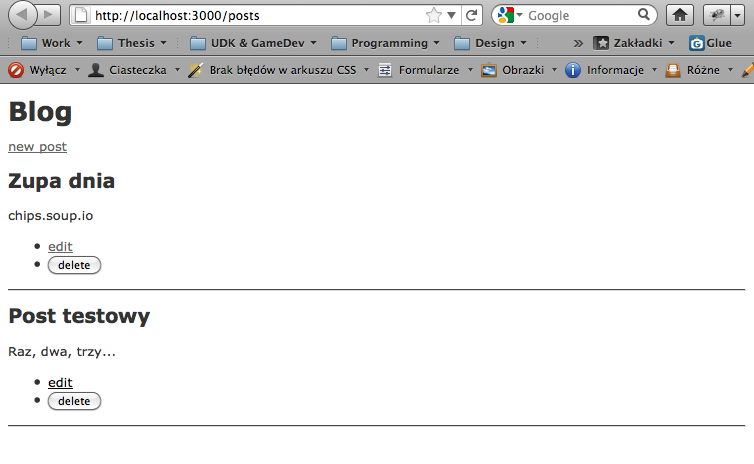
\includegraphics[width=\linewidth]{images/blog.png}
			\caption{Aplikacja testowa - wyświetlanie artykułów}
			\label{blog_view}
		\end{center}
	\end{figure}
	
	\begin{figure}[h!]
		\begin{center}
			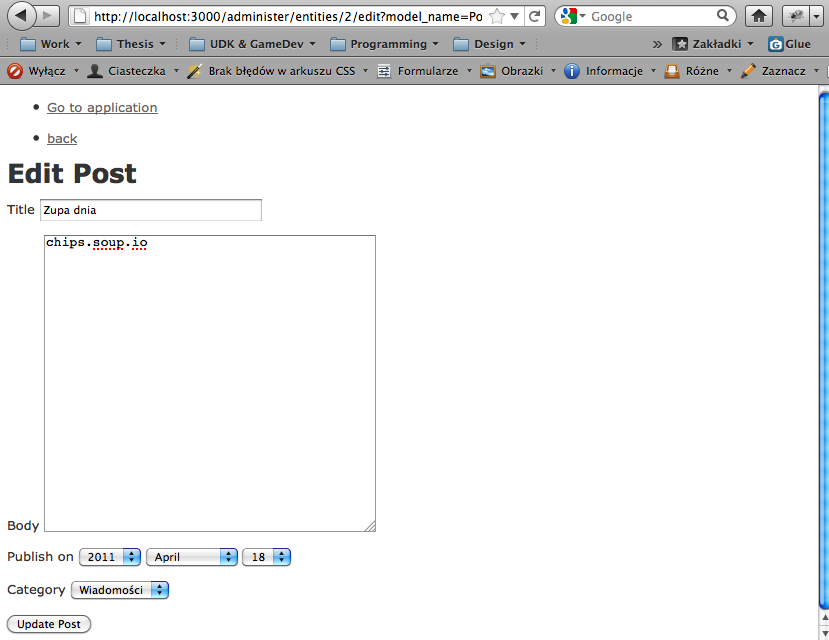
\includegraphics[width=\linewidth]{images/administer_edit.png}
			\caption{administer - edycja rekordu}
			\label{administer_edit}
		\end{center}
	\end{figure}
  
  % lepsza nazwa
  \subsection{Konfiguracja zależności testowych}
    % aplikacja testowa powinna kożystać ze źródeł testowanego gema, nie z jego release
    % Test dependencies - warto coś o tym napisać?
    
  % zdecydowanie zmień nazwę tej sekcji 
  \subsection{Implementacja konkretnej funkcji od A do Z}
    % screen z listą tiketów
    % dokładny opis całego procesu + wycinki kodu źródłowego dla konkretnego tiketa
  
  \section{Wnioski}
